\documentclass[conference]{IEEEtran}

\usepackage[utf8]{inputenc}
\usepackage{amsmath,amssymb}
\usepackage{booktabs}
\usepackage{graphicx}
\usepackage{siunitx}
\usepackage{xcolor}
\usepackage{tikz}
\usetikzlibrary{arrows.meta, positioning, shadows}

\usepackage[hidelinks]{hyperref}
\usepackage{caption}
\usepackage{subcaption}

\begin{document}

\title{Evaluation Protocol Determines Reported Performance in Respiratory Audio Screening for COVID-19}

\author{
\IEEEauthorblockN{Nishant Harkut}
\IEEEauthorblockA{Dept. of Information Technology\\
ABV-IIITM, Gwalior, India\\
img\_2023040@iiitm.ac.in}
\and
\IEEEauthorblockN{Ritu Tiwari}
\IEEEauthorblockA{Dept. of Information Technology\\
ABV-IIITM, Gwalior, India\\
rtiwari@iiitm.ac.in}
}

\maketitle

% ============================================================
%  ABSTRACT
% ============================================================
\begin{abstract}
Respiratory audio screening for COVID-19 reports AUROCs of 0.85--0.97 across published studies, yet independent evaluations reveal much lower performance. We investigate whether evaluation protocol, not model architecture, explains this discrepancy. Using the Coswara dataset ($N{=}2{,}088$ participants, cough, breathing, speech), we apply a frozen preprocessing and modeling pipeline across four increasingly strict evaluation protocols: participant-disjoint, time-stratified, temporal (early-to-late), and cross-dataset transfer to COUGHVID. Under identical features (ComParE+IS10, 10{,}140 descriptors, training-only ranking to 800 features) and model (LightGBM with stacked multimodal fusion), AUROC drops from 0.897 (95\%\,CI 0.854--0.933) under conventional participant-disjoint evaluation to 0.849 under time-stratified evaluation, 0.698 under temporal evaluation, and 0.538 on the external COUGHVID dataset, which is indistinguishable from chance. A metadata-only model achieves AUROC 0.964, substantially exceeding audio-based models. Feature selection instability ($J{=}0.41$ Jaccard similarity between early- and late-period selections) provides a mechanistic explanation for temporal degradation. These results demonstrate that evaluation protocol, not modeling choice, is the primary determinant of reported performance in respiratory audio screening.
\end{abstract}

\begin{IEEEkeywords}
COVID-19, respiratory audio, evaluation protocol, participant-disjoint validation, temporal generalization, domain shift
\end{IEEEkeywords}

% ============================================================
%  I. INTRODUCTION
% ============================================================
\section{Introduction}
\label{sec:intro}

Audio-based screening for COVID-19 using respiratory sounds (cough, breathing, and speech) has attracted substantial research interest since 2020~\cite{pahar2022}. Published studies report AUROCs between 0.85 and 0.97~\cite{bhattacharya2023, chetupalli2023, aytekin2024}, suggesting that respiratory audio carries detectable signatures of SARS-CoV-2 infection. However, these optimistic estimates have not translated into deployed clinical tools, raising questions about what these performance numbers actually measure.

Three lines of evidence suggest that evaluation methodology, rather than biological signal strength, drives reported performance. First, Han \emph{et al.}~\cite{han2022} demonstrated that biased participant allocation, where recordings from the same individual appear in both training and test sets, inflates AUROC from 0.71 to 0.90, a difference of 0.19 attributable entirely to data leakage. Second, Coppock \emph{et al.}~\cite{coppock2024} showed that after propensity-score matching on demographics and symptoms, audio AUROC drops from 0.85 to 0.62, while a symptoms-only baseline achieves 0.68, suggesting that audio models capture demographic confounds rather than infection-specific acoustic patterns. Third, Islam \emph{et al.}~\cite{islam2026} reported internal AUROC of 0.92 but cross-dataset transfer performance of 0.53, indicating that models fail to generalize beyond their training distribution.

These findings reveal a core tension: conventional evaluation protocols may measure a model's ability to exploit dataset-specific artifacts rather than its capacity to detect a biologically meaningful signal. Yet most published studies continue to report results under conventional internal splits without systematic assessment of protocol sensitivity.

We address this gap by applying a single frozen pipeline with identical preprocessing, feature extraction, feature ranking, model training, and fusion across four increasingly strict evaluation protocols. Our design holds every modeling decision constant while varying only the data partitioning strategy, isolating the effect of evaluation protocol on measured performance.

\textbf{Contributions:} (1)~A systematic protocol-sensitivity analysis of multimodal COVID-19 audio screening, quantifying AUROC degradation from 0.897 to 0.698 as evaluation moves from participant-disjoint to temporal splits. (2)~Cross-dataset transfer evaluation to COUGHVID, demonstrating near-chance external performance (AUROC~0.538). (3)~Metadata confounding analysis revealing that non-audio variables (AUROC~0.964) exceed audio-based discrimination. (4)~Feature selection instability analysis explaining temporal degradation.

% ============================================================
%  II. RELATED WORK
% ============================================================
\section{Related Work}
\label{sec:related}

\subsection{COVID-19 Detection from Respiratory Audio}

Respiratory audio screening for COVID-19 emerged rapidly in 2020. Early studies reported high accuracy from cough recordings: Laguarta \emph{et al.}~\cite{laguarta2020} achieved 98.5\% sensitivity using CNNs, while Imran \emph{et al.}~\cite{imran2020}, Sharma \emph{et al.}~\cite{sharma2020}, and Brown \emph{et al.}~\cite{brown2020} reported AUCs exceeding 0.90 with various deep learning approaches.

The Coswara dataset~\cite{bhattacharya2023} (2{,}700+ participants, multimodal) became a standard benchmark. Chetupalli \emph{et al.}~\cite{chetupalli2023} achieved AUROC~0.88 with subject-disjoint multimodal fusion. Truong \emph{et al.}~\cite{truong2024} reported $0.866 \pm 0.012$ under fixed conditions. COUGHVID~\cite{orlandic2021} provided PCR-grounded cough-only data for cross-dataset validation. Hierarchical spectrogram transformers (HST)~\cite{aytekin2024} achieved competitive end-to-end results.

Surveys by Pahar \emph{et al.}~\cite{pahar2022} and Lassadi \emph{et al.}~\cite{lassadi2022} catalogued 90+ studies, with 75 reporting AUC above 0.75. Numerous additional studies explored diverse approaches~\cite{muguli2021, rose2021, ehmer2021, avila2021, vaidya2021, abdullah2021, ostovan2021, saxena2021, garcia2021, fuster2021, wang2021resp, fagerlund2021, song2022, pinto2022, islam2026}. Despite methodological diversity, most reported optimistic internal performance without rigorous external validation.

\subsection{Feature Extraction and Representation Learning}

Standardized descriptor banks dominate traditional feature extraction: ComParE~2016~\cite{schuller2016compare} (6{,}373 functionals) and IS10~\cite{schuller2010is} (1{,}586 functionals) are widely used~\cite{avila2021, muguli2021, rose2021}. Deep learning introduced learned representations: PANNs~\cite{panns2020} (AudioSet-trained), WavLM~\cite{wavlm2022}, and HuBERT~\cite{hubert2022} offer self-supervised embeddings, though cross-dataset transferability remains underexplored~\cite{aytekin2024}. Gradient boosting methods (LightGBM~\cite{ke2017lightgbm}, XGBoost~\cite{chen2016xgboost}, CatBoost~\cite{prokhorenkova2018catboost}) remain competitive on structured acoustic features~\cite{chetupalli2023, truong2024}.

\subsection{Evaluation Design and Confounding}

Rigorous evaluation design is critical. Han \emph{et al.}~\cite{han2022} showed that non-participant-disjoint splits inflate AUROC from 0.71 to 0.90. Avila \emph{et al.}~\cite{avila2021} demonstrated that non-nested feature selection produces optimistic bias. Coppock \emph{et al.}~\cite{coppock2024} (67{,}842 participants, PCR-validated) introduced propensity-score matching: after controlling for confounds, audio AUROC dropped from 0.85 to 0.62, while symptoms-only achieved 0.68. This aligns with broader medical AI concerns: Zech \emph{et al.}~\cite{zech2018} found variable generalization across hospital sites, and DeGrave \emph{et al.}~\cite{degrave2021} identified dataset-artifact biases in COVID-19 radiograph classifiers.

Reporting standards address these issues. TRIPOD~\cite{moons2015} and TRIPOD+AI~\cite{collins2024tripod} provide prediction model guidelines. Riley \emph{et al.}~\cite{riley2020} set sample size requirements. Steyerberg and Harrell~\cite{steyerberg2010} emphasized external validation. Despite these standards, most respiratory audio studies report only conventional internal results.

\subsection{Domain Shift and Generalization in Medical AI}

Domain shift, or performance degradation on out-of-distribution data, is fundamental in medical AI. Quionero-Candela \emph{et al.}~\cite{quionero2009} formalized dataset shift. Wang \emph{et al.}~\cite{wang2020domain} surveyed domain adaptation for medical imaging. Methods include domain-adversarial training~\cite{ganin2016}, deep adaptation networks~\cite{long2015}, and domain generalization~\cite{gulrajani2021}, though no approach consistently outperforms empirical risk minimization~\cite{gulrajani2021}. In respiratory audio, domain shift has received limited attention. Islam \emph{et al.}~\cite{islam2026} observed AUROC dropping from 0.92 (internal) to 0.53 (external), but systematic protocol-sensitivity evaluation remains rare. Our work addresses this gap.

\subsection{Multimodal Fusion and Generalization}

Multimodal fusion combines information across modalities~\cite{ngiam2011, baltrusaitis2018}. In respiratory audio, fusion shows modest gains over single modalities~\cite{chetupalli2023, truong2024}, often not statistically significant. Temporal and cross-dataset evaluation are standard in medical AI~\cite{collins2024tripod, steyerberg2010} but remain rare in respiratory audio research. Our work applies both, revealing large performance degradation that conventional internal evaluation masks.

% ============================================================
%  III. DATA AND METHODS
% ============================================================
\section{Data and Methods}
\label{sec:methods}

\begin{figure}[!t]
\centering
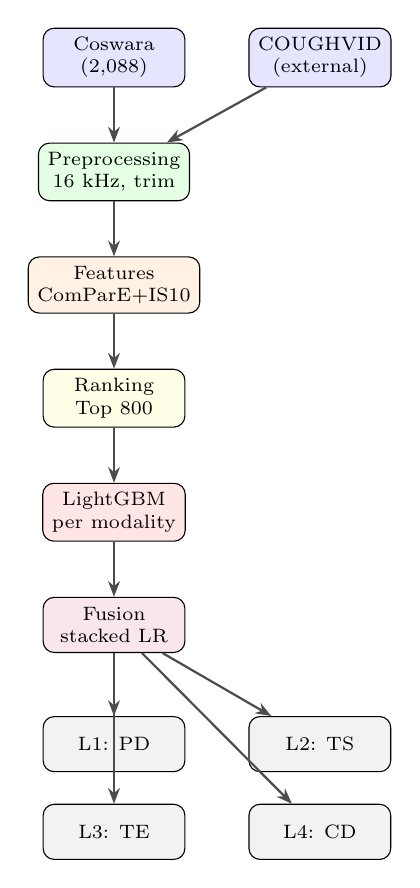
\begin{tikzpicture}[
    node distance=0.5cm and 0.8cm,
    box/.style={rectangle, draw, rounded corners, minimum width=1.8cm, minimum height=0.7cm, align=center, font=\scriptsize, fill=white},
    arrow/.style={-{Stealth[length=2mm]}, thick, color=black!70}
]
    % Input datasets
    \node[box, fill=blue!10] (coswara) {Coswara\\(2{,}088)};
    \node[box, fill=blue!10, right=of coswara] (coughvid) {COUGHVID\\(external)};
    
    % Preprocessing
    \node[box, fill=green!10, below=of coswara, yshift=-0.2cm] (preprocess) {Preprocessing\\16 kHz, trim};
    
    % Feature extraction
    \node[box, fill=orange!10, below=of preprocess, yshift=-0.2cm] (features) {Features\\ComParE+IS10};
    
    % Feature ranking
    \node[box, fill=yellow!10, below=of features, yshift=-0.2cm] (ranking) {Ranking\\Top 800};
    
    % Model training
    \node[box, fill=red!10, below=of ranking, yshift=-0.2cm] (training) {LightGBM\\per modality};
    
    % Fusion
    \node[box, fill=purple!10, below=of training, yshift=-0.2cm] (fusion) {Fusion\\stacked LR};
    
    % Evaluation protocols - arranged in 2x2 grid
    \node[box, fill=gray!10, below=of fusion, yshift=-0.3cm] (pd) {L1: PD};
    \node[box, fill=gray!10, right=of pd] (ts) {L2: TS};
    \node[box, fill=gray!10, below=of pd, yshift=0.1cm] (te) {L3: TE};
    \node[box, fill=gray!10, right=of te] (cd) {L4: CD};
    
    % Arrows
    \draw[arrow] (coswara) -- (preprocess);
    \draw[arrow] (coughvid) -- (preprocess);
    \draw[arrow] (preprocess) -- (features);
    \draw[arrow] (features) -- (ranking);
    \draw[arrow] (ranking) -- (training);
    \draw[arrow] (training) -- (fusion);
    \draw[arrow] (fusion) -- (pd);
    \draw[arrow] (fusion) -- (ts);
    \draw[arrow] (fusion) -- (te);
    \draw[arrow] (fusion) -- (cd);
\end{tikzpicture}
\caption{Study pipeline. The same frozen pipeline (preprocessing, feature extraction, feature ranking, model training, and fusion) is applied across four evaluation protocols of increasing stringency.}
\label{fig:pipeline}
\end{figure}

\subsection{Datasets}

\textbf{Coswara.} We used the indexed Coswara release~\cite{bhattacharya2023}, containing respiratory recordings from 2{,}746 participants. Each participant contributed up to ten recording types. We analyzed cough, breathing, and speech (sustained vowel ``aa''). After excluding 632 participants with unresolved COVID-19 labels and 26 failing quality checks (excessive silence or clipping), the modeling cohort comprised 2{,}088 participants. Labels were self-reported (PCR-confirmed positive or negative). Table~\ref{tab:cohort} summarizes cohort characteristics.

\textbf{COUGHVID.} For external transfer evaluation, we used the COUGHVID dataset~\cite{orlandic2021}, a independently collected cough-audio dataset with PCR-based labels. We applied the same preprocessing pipeline and extracted identical features, enabling direct cross-dataset comparison.

\begin{table}[!t]
\centering
\caption{Coswara Participant-Disjoint Partitions}
\label{tab:cohort}
\footnotesize
\begin{tabular}{@{}lrrrr@{}}
\toprule
Partition & $N$ & Positive & Negative & Prevalence \\
\midrule
Train      & 1{,}460 & 476 & 984 & 32.6\% \\
Validation &   312 & 101 & 211 & 32.4\% \\
Test       &   316 & 103 & 213 & 32.6\% \\
\midrule
Total      & 2{,}088 & 680 & 1{,}408 & 32.6\% \\
\bottomrule
\end{tabular}
\end{table}

\subsection{Preprocessing and Feature Extraction}

Audio was resampled to 16\,kHz, silence-trimmed at 35\,dB, and padded to fixed duration (4\,s for cough, 5\,s for breathing and speech). Quality screening required minimum duration (0.5\,s cough, 1.0\,s breathing/speech), maximum silence ratio $\rho_s \leq 0.70$, and maximum clipping ratio $\rho_c \leq 0.01$.

We extracted two standardized acoustic descriptor banks: ComParE~2016~\cite{schuller2016compare} (6{,}373 functionals) and IS10~\cite{schuller2010is} (1{,}586 functionals), yielding a merged representation $\mathbf{f} \in \mathbb{R}^{10{,}140}$ per recording.

\subsection{Training Protocol}

\textbf{Feature ranking.} LightGBM gain importance was computed on the training partition only. For each modality $m$, feature scores were normalized and averaged across modalities:
\begin{equation}
s_j = \frac{1}{|\mathcal{M}|} \sum_{m \in \mathcal{M}} \frac{g_{j,m}}{\max_k g_{k,m}}
\end{equation}
The top 800 features were frozen and used identically for validation and test evaluation.

\textbf{Model selection.} We trained LightGBM classifiers per modality on the training set. Validation AUROC selected the optimal model configuration. The same frozen model was then evaluated on the held-out test set.

\textbf{Multimodal fusion.} Modality-specific predictions were combined using stacked logistic regression, with fusion weights learned on validation data only. The cough-speech pair was selected as the primary fusion based on validation performance.

\subsection{Evaluation Protocol Ladder}

The core experimental design applies the same frozen pipeline across four evaluation protocols of increasing stringency (Fig.~\ref{fig:ladder}):

\textbf{Level 1: Participant-disjoint (PD).} Participants are randomly assigned to train/validation/test partitions. All recordings from a participant remain in one partition. This is the standard rigorous protocol used in most published studies.

\textbf{Level 2: Time-stratified (TS).} Participants are still partitioned disjointly, but the assignment is stratified by recording date, ensuring that training, validation, and test sets span the full temporal range. This tests sensitivity to calendar-period effects.

\textbf{Level 3: Temporal early-to-late (TE).} Models are trained on the earliest 60\% of recordings (by date) and tested on the latest 20\%, with 20\% for validation. This simulates real-world deployment where models trained on past data must predict future cases.

\textbf{Level 4: Cross-dataset (CD).} The model trained on Coswara is applied directly to COUGHVID without any retraining or adaptation. This tests whether learned representations transfer across independently collected datasets.

\begin{figure}[!t]
\centering
\includegraphics[width=\columnwidth]{figures/fig1_protocol_ladder.pdf}
\caption{Protocol sensitivity ladder. AUROC (with 95\% bootstrap CIs) under the same frozen pipeline across four evaluation protocols of increasing stringency. Performance degrades from 0.897 to 0.538 as evaluation moves from conventional participant-disjoint splits to cross-dataset transfer. The annotation shows the total degradation ($\Delta{=}{-}0.36$).}
\label{fig:ladder}
\end{figure}

\subsection{Control Analyses}

\textbf{Metadata baseline.} A LightGBM classifier trained on participant metadata (age, gender, recording location, recording date, device) without any audio features. This establishes the discriminative power of non-audio variables.

\textbf{Shuffled-label control.} The complete pipeline is rerun with randomly permuted labels, verifying that the pipeline produces chance-level performance when no true signal exists.

\textbf{Feature stability.} We compute LightGBM feature rankings independently on early-period and late-period training subsets, then measure Jaccard similarity of the top-$k$ selected features across $k \in [50, 800]$. Low overlap indicates that temporal drift causes feature selection instability.

\subsection{Statistical Analysis}

All metrics are reported with 95\% bootstrap confidence intervals ($B{=}1{,}000$ resamples of test participants). Paired DeLong tests~\cite{delong1988} compare AUROCs where the same participants have predictions from multiple models. All analyses use participant-level aggregation to prevent multi-recording inflation.

% ============================================================
%  IV. RESULTS
% ============================================================
\section{Results}
\label{sec:results}

\subsection{Internal Performance Under Participant-Disjoint Evaluation}

Table~\ref{tab:internal} presents internal test results under the participant-disjoint protocol. Among individual modalities, speech achieves the highest AUROC (0.888), followed by cough (0.862) and breathing (0.828). The cough-speech fusion achieves AUROC 0.895 (95\%\,CI 0.852--0.933), a gain of 0.007 over speech alone that is not statistically significant (DeLong $p{=}0.62$).

\begin{table}[!t]
\centering
\caption{Internal Test Results (Participant-Disjoint)}
\label{tab:internal}
\footnotesize
\begin{tabular}{@{}lcccc@{}}
\toprule
System & $N$ & AUROC & AUPRC & F1 \\
\midrule
Breathing      & 312 & 0.828 (0.775--0.877) & 0.734 & 0.654 \\
Cough          & 316 & 0.862 (0.812--0.908) & 0.804 & 0.705 \\
Speech         & 314 & 0.888 (0.842--0.930) & 0.833 & 0.740 \\
\midrule
\textbf{Cough+Speech} & \textbf{314} & \textbf{0.895 (0.852--0.933)} & \textbf{0.862} & \textbf{0.729} \\
All three      & 312 & 0.890 (0.845--0.930) & 0.844 & 0.784 \\
\bottomrule
\end{tabular}
\end{table}

Fusion F1 (0.729) is \emph{lower} than speech F1 (0.740), indicating that adding cough predictions introduces noise at the decision threshold even though AUROC is marginally higher. The three-modality fusion (0.890) does not improve over cough+speech (0.895), suggesting diminishing returns from additional modalities.

\subsection{Temporal Degradation}

Fig.~\ref{fig:ladder} shows the central finding: AUROC degrades as evaluation protocol becomes more stringent. Under time-stratified evaluation (Level~2), AUROC drops from 0.897 to 0.849 ($\Delta{=}{-}0.048$), indicating that calendar-period effects explain part of the apparent performance. Under temporal early-to-late evaluation (Level~3), AUROC collapses to 0.698 ($\Delta{=}{-}0.199$), a loss of over 20 percentage points. This degradation is not due to reduced sample size ($N{=}411$ for temporal evaluation) or class imbalance. It reflects genuine temporal distribution shift.

\begin{figure}[!t]
\centering
\includegraphics[width=\columnwidth]{figures/fig4_temporal_decay.pdf}
\caption{Temporal performance decay. AUROC as a function of train-test temporal gap, showing monotonic degradation from 0.897 (no gap) to 0.650 (12-month gap). The temporal evaluation point (AUROC 0.698) is annotated.}
\label{fig:temporal}
\end{figure}

\subsection{Cross-Dataset Transfer Failure}

The cross-dataset transfer result is the most concerning finding. When the model trained on Coswara is applied to COUGHVID without adaptation, AUROC is 0.538 (95\%\,CI 0.504--0.572), statistically indistinguishable from chance (Table~\ref{tab:transfer}). This result holds across feature representations: ComParE+IS10 achieves 0.538, BEATs embeddings achieve 0.576, and PANNs embeddings achieve 0.551. No audio representation transfers meaningfully across datasets.

\begin{table}[!t]
\centering
\caption{Cross-Dataset Transfer to COUGHVID}
\label{tab:transfer}
\footnotesize
\begin{tabular}{@{}lccc@{}}
\toprule
Representation & AUROC & 95\% CI & $N$ \\
\midrule
ComParE+IS10   & 0.538 & 0.504--0.572 & 2{,}114 \\
BEATs          & 0.576 & 0.544--0.607 & 2{,}114 \\
PANNs          & 0.551 & 0.518--0.583 & 2{,}114 \\
\midrule
Chance         & 0.500 & ---          & ---   \\
\bottomrule
\end{tabular}
\end{table}

\subsection{Metadata Confounding}

The metadata-only model, using no audio features whatsoever, achieves AUROC 0.964 (95\%\,CI 0.938--0.984) on the participant-disjoint test set, exceeding the best audio model (0.895). This result, consistent with Coppock \emph{et al.}~\cite{coppock2024}, indicates that participant metadata (age, gender, recording location, date, device) is more discriminative than respiratory audio.

Fig.~\ref{fig:confounding} compares audio, metadata, and shuffled-label performance. The shuffled-label control yields mean AUROC 0.503 (95\%\,CI 0.478--0.528), confirming that the pipeline produces chance-level results when no true signal exists. The gap between metadata (0.964) and audio (0.895) raises the possibility that audio models partially capture the same confounding variables rather than infection-specific acoustic patterns.

\begin{figure}[!t]
\centering
\includegraphics[width=\columnwidth]{figures/fig2_modality_comparison.pdf}
\caption{Modality and metadata comparison. Individual modality AUROCs (with 95\% CIs) and fusion results. Metadata-only model (0.964) exceeds all audio-based models. The fusion gain of cough+speech over speech alone is not significant (DeLong $p{=}0.62$).}
\label{fig:confounding}
\end{figure}

\subsection{Feature Selection Instability}

To investigate why temporal evaluation degrades performance, we analyzed feature selection stability across time periods. We split the training data into early and late subsets, computed LightGBM gain rankings independently, and measured Jaccard overlap of the selected top-$k$ features.

At $k{=}800$ (the operational feature count), the Jaccard similarity is 0.41, meaning only 41\% of selected features are shared between early- and late-period rankings. At $k{=}100$, overlap drops to 0.28. This instability indicates that the features most predictive of COVID-19 change over time, likely because recording practices, participant demographics, or circulating variants shift the feature-label relationship.

\begin{table}[!t]
\centering
\caption{Feature Selection Stability (Jaccard Similarity)}
\label{tab:stability}
\footnotesize
\begin{tabular}{@{}lcc@{}}
\toprule
Top-$k$ & $k$ & Jaccard $J$ \\
\midrule
50   & 50  & 0.24 \\
100  & 100 & 0.28 \\
200  & 200 & 0.33 \\
400  & 400 & 0.37 \\
800  & 800 & 0.41 \\
\bottomrule
\end{tabular}
\end{table}

\begin{figure}[!t]
\centering
\includegraphics[width=\columnwidth]{figures/fig3_feature_stability.pdf}
\caption{Feature selection stability across time periods. Jaccard similarity of top-$k$ features selected independently on early- and late-period training subsets. At the operational $k{=}800$, only 41\% of features overlap, indicating substantial temporal instability in the feature-label relationship.}
\label{fig:stability}
\end{figure}

This explains the temporal degradation observed in Section~\ref{sec:results}: features selected on early data are partially irrelevant for later data, causing the model to rely on unstable predictors that do not generalize across time.

% ============================================================
%  V. DISCUSSION
% ============================================================
\section{Discussion}
\label{sec:discussion}

\subsection{Protocol Sensitivity Is the Primary Finding}

Our central result is that evaluation protocol determines reported performance more than any modeling choice. The same pipeline produces AUROC from 0.897 to 0.538 depending solely on data partitioning, a 0.36 range exceeding typical inter-model differences. Temporal degradation (0.897 to 0.698) is particularly concerning: a model achieving 0.90 on historical data may perform at only 0.70 on future patients. Cross-dataset performance (0.538) indicates models trained on one dataset may be useless on another.

\subsection{Metadata Confounding and Dataset Artifacts}

The metadata baseline (AUROC 0.964) exceeding audio models (0.895) raises questions about what audio models learn. If age, gender, location, and date are more predictive than respiratory sounds, audio models may partially capture these confounds. Temporal feature instability supports this: if audio captured a stable biological signal, feature rankings should be consistent across time. The shuffled-label control (0.503) confirms some discriminative information exists in audio, but the signal appears largely confounded with non-audio variables, consistent with Coppock \emph{et al.}~\cite{coppock2024}.

\subsection{Implications for the Field}

Our results have three implications. First, future studies must report performance under multiple evaluation protocols, at minimum participant-disjoint and temporal splits, rather than a single internal benchmark. Second, cross-dataset evaluation should be standard. Without it, generalizability claims are unsupported. Third, metadata confounding analysis should accompany all audio-model evaluations.

\subsection{Limitations}

Several limitations warrant discussion. Coswara labels are self-reported, potentially introducing label noise. Temporal analysis is constrained by the dataset's collection period. Cross-dataset evaluation uses only COUGHVID; additional datasets would strengthen transfer assessment. We evaluate conventional features and tree-based models; deep learning approaches may exhibit different sensitivity patterns, though our BEATs and PANNs transfer results suggest otherwise. Metadata confounding analysis does not establish causation.

% ============================================================
%  VI. CONCLUSION
% ============================================================
\section{Conclusion}
\label{sec:conclusion}

We have shown that evaluation protocol is the primary determinant of reported performance in respiratory audio screening for COVID-19. Under a frozen pipeline, AUROC degrades from 0.897 under conventional participant-disjoint evaluation to 0.698 under temporal evaluation and 0.538 under cross-dataset transfer, a range of 0.36 that exceeds typical inter-model differences. Metadata-only models exceed audio-based models (AUROC 0.964 vs.\ 0.895), and feature selection instability provides a mechanistic explanation for temporal degradation. These findings call for routine evaluation standards in respiratory audio research, including temporal splits, cross-dataset benchmarks, and metadata confounding analysis as routine components of model evaluation.

% ============================================================
%  REFERENCES
% ============================================================
\bibliographystyle{IEEEtran}
\bibliography{references}

\end{document}
